% Created 2021-02-16 Tue 23:27
% Intended LaTeX compiler: pdflatex
\documentclass[11pt]{article}
\usepackage[utf8]{inputenc}
\usepackage[T1]{fontenc}
\usepackage{graphicx}
\usepackage{grffile}
\usepackage{longtable}
\usepackage{wrapfig}
\usepackage{rotating}
\usepackage[normalem]{ulem}
\usepackage{amsmath}
\usepackage{textcomp}
\usepackage{amssymb}
\usepackage{capt-of}
\usepackage{hyperref}
\usepackage{minted}
\setlength\parindent{0pt}
\usepackage[bottom]{footmisc}
\author{Trent Fridey}
\date{\today}
\title{Task 1}
\hypersetup{
 pdfauthor={Trent Fridey},
 pdftitle={Task 1},
 pdfkeywords={},
 pdfsubject={},
 pdfcreator={Emacs 27.1 (Org mode 9.4)}, 
 pdflang={English}}
\begin{document}

\maketitle
\tableofcontents

\pagebreak

\section{Part 1}
\label{sec:org547f5d1}

A variational quantum circuit that is able to generate the most general 1-qubit state, starting from the initial state \(|0\rangle\) is the following:

\begin{center}
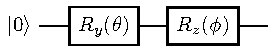
\includegraphics[width=.9\linewidth]{circuits/variational/variational.pdf}
\end{center}

\textbf{\textbf{Proof}}:

A general state on the Bloch sphere can be parameterized by two angles, \(\theta \in [0,\pi)\) and \(\phi \in [0,2\pi)\), as:

\begin{equation*}
| \theta, \phi \rangle =
\begin{bmatrix}
\cos(\theta/2) \\
e^{i\phi}\sin(\theta/2)
\end{bmatrix}
\end{equation*}


The matrix representation of our circuit is:

\begin{align*}
R_z(\phi)R_y(\theta) &= 
\begin{bmatrix}
\cos(\theta/2) & -\sin(\theta/2) \\
\sin(\theta/2) & \cos(\theta/2)
\end{bmatrix}
\begin{bmatrix}
e^{-i\phi/2} & 0 \\
0 & e^{i\phi/2}  \\
\end{bmatrix} \\
&=
\begin{bmatrix}
\cos(\theta/2)e^{-i\phi/2} & -\sin(\theta/2)e^{i\phi/2} \\
\sin(\theta/2)e^{-i\phi/2} & \cos(\theta/2)e^{i\phi/2}
\end{bmatrix}
\end{align*}

Our initial state is \(|0\rangle\). The resulting state after the circuit is:

\begin{align*}
R_z(\phi)R_y(\theta)|0\rangle &= 
\begin{bmatrix}
\cos(\theta/2)e^{-i\phi/2} & -\sin(\theta/2)e^{i\phi/2} \\
\sin(\theta/2)e^{-i\phi/2} & \cos(\theta/2)e^{i\phi/2}
\end{bmatrix}
\begin{bmatrix}
1 \\
0
\end{bmatrix} \\
&=
e^{-i\phi/2}\begin{bmatrix}
\cos(\theta/2) \\
e^{i\phi}\sin(\theta/2)
\end{bmatrix}
=
| \theta, \phi \rangle 
\end{align*}


which is equivalent to \(|\theta,\phi\rangle\) modulo a global phase. \(\blacksquare\)

\pagebreak

\section{Part 2}
\label{sec:org47932fd}

Let \(|r\rangle\) be a random 1-qubit state. From above, we know that it can be written as \(|r\rangle = |\theta_0,\phi_0\rangle\) for some angles \(\theta_0, \phi_0\). Since we don't know the angles ahead of time, we can't find the random state by just tuning our gates to \(R_z(\phi_0)\) and \(R_y(\theta_0)\). Instead, we can use the SWAP test and machine learning to discover the angles. The principle behind this approach is minimizing a cost function in terms of the overlap between the random state \(|r\rangle\) and the controlled state \(|\theta, \phi\rangle\)

\begin{equation*}
\text{cost} \propto 1-|\langle r | \theta, \phi \rangle|^2
\end{equation*}

We can implement this cost function using the SWAP test as in the following circuit:

\begin{center}
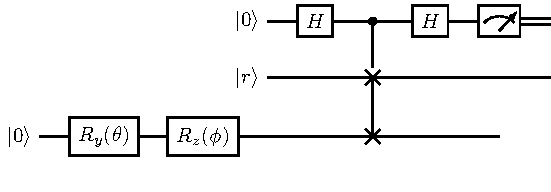
\includegraphics[width=.9\linewidth]{circuits/total/total.pdf}
\end{center}

\textbf{\textbf{Proof}}:

The wavefunction of the system immediately before measurement is:


\[
\frac{1}{2}|0\rangle \left( |\theta,\phi \rangle|r\rangle + |r\rangle|\theta_{},\phi_{}\rangle \right) +
 \frac{1}{2}|1\rangle \left(|\theta,\phi\rangle|r\rangle - |r\rangle|\theta_{},\phi\rangle \right)
\]

Let \(M\) be the value measured of the ancilla qubit, in the \(z\) - basis, \(\{|0\rangle, |1\rangle \}\), returning the value 0 or 1 respectively. Suppose we run the circuit \(n\) times, so that we obtain a set of measurements \(\{ M_i \}_{i=1}^n\). Then in the limit \(n\to\infty\), we can compute the overlap:

\begin{equation*}
\lim_{n\to\infty } \left( 1 - \frac{2}{n}\sum_{i=1}^n M_i \right) = |\langle r | \theta, \phi \rangle|^2
\end{equation*}


The extension to the cost function is straightforward \(\blacksquare\).


We then run this circuit many times \((n \gg 1)\) so that we can approach the limiting value as mentioned in the proof. Once we have the resulting measurements, the optimal angles \(\theta_0\), \(\phi_0\) are the solution to the minimization problem:

\begin{equation*}
(\theta_{0}, \phi_{0}) = \arg\min_{(\theta, \phi)} \frac{2}{n}\sum_{i=1}^{n} M_i
\end{equation*}

We can solve this via an appropriate minimization algorithm.

\pagebreak

\subsection{Implementation}
\label{sec:org4ed7ace}


We can implement the circuit and the optimization using the Pennylane Python library:

\begin{minted}[]{python}
import pennylane as qml
from pennylane import numpy as np
\end{minted}

For the purposes of illustration, in this implementation we let the random state be \(|r\rangle = |\theta_0=\pi/8, \phi_0=\pi/4 \rangle\). In reality, in order to be actually random, we would not know this ahead of time.

\begin{minted}[]{python}
t_0 = 0.125*np.pi # ~ 0.3927
p_0 = 0.25*np.pi  # ~ 0.7854
\end{minted}

Now we are ready to implement our circuit. We use \texttt{QubitStateVector} to define the random state: 

\begin{minted}[]{python}
num_shots = 1000
dev = qml.device('default.qubit', wires=3, shots=num_shots)

@qml.qnode(dev)
def var_swap(params):
  # random state preparation
  qml.QubitStateVector([
      np.cos(t_0/2.),
      np.sqrt(0.5)*(1+1j)*np.sin(t_0/2.)
  ], wires=1)
  # actual circuit follows:
  qml.RY(params[0], wires=2)
  qml.RZ(params[1], wires=2)
  qml.Hadamard(wires=0)
  qml.CSWAP(wires=[0,1,2])
  qml.Hadamard(wires=0)
  return qml.sample(qml.PauliZ(0))
\end{minted}


Now we set up the optimizer.
Define the cost function:

\begin{minted}[]{python}
def cost(params):
    return 1-(1./num_shots)*np.sum(var_swap(params))
\end{minted}

Define the initial parameters:

\begin{minted}[]{python}
params = np.array([0.,0.])
\end{minted}

Now we define the optimization algorithm.
Because our cost function has a stochastic output (via the call to \texttt{qml.sample}), we are limited to using \emph{gradient-free} methods of optimization.
In this case we can use Rotosolve via the \texttt{RotosolveOptimizer}.\footnote{Pennylane also has an API for the \href{https://pennylane.readthedocs.io/en/stable/code/api/pennylane.RotoselectOptimizer.html}{RotoselectOptimizer}, which not only can find the best \(\theta, \phi\) minimizing the cost function, but can also find the best rotation gates for us! However, we already know the best set of rotation gates -- they are the gates we used to prepare the "random" state.}

\begin{minted}[]{python}
opt = qml.RotosolveOptimizer()

\end{minted}

So with that we are ready to run the optimization:

\begin{minted}[]{python}
steps = 100
best_cost = [cost(params)]
best_params = params
for i in range(steps):
  params = opt.step(cost, params)
  new_cost = cost(params)
  if(new_cost < best_cost[-1]):
    best_params = params
  best_cost.append(new_cost)

print(best_params)
\end{minted}

\begin{verbatim}
[0.40703541 0.93070817]
\end{verbatim}


The optimization gives \(\theta =\) \texttt{0.40703540572409325} and \(\phi =\) \texttt{0.9307081740331506}, which differs from the actual best parameters by:

$\theta - \pi/8 = 0.0143, \phi - \pi/4 = 0.145$


\pagebreak

We visually check the progression of our optimizer with a plot of cost-vs-steps:

\begin{center}
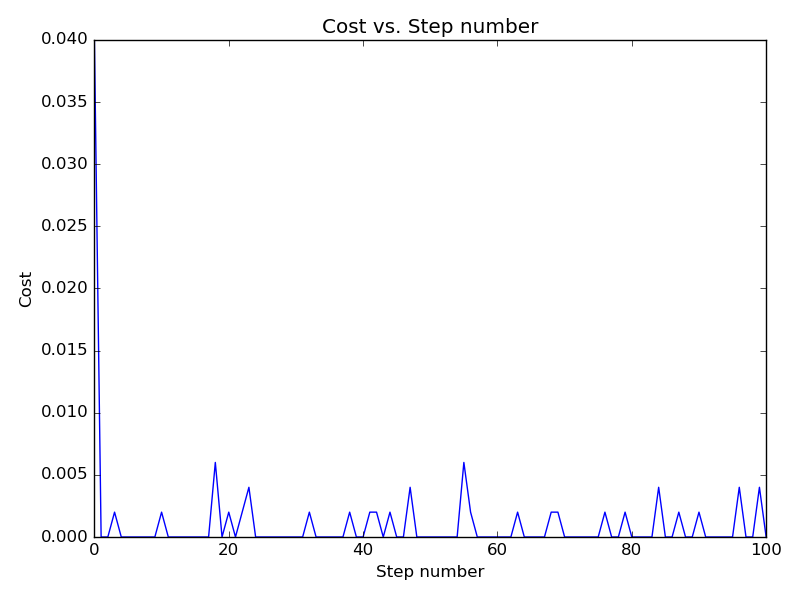
\includegraphics[width=.9\linewidth]{images/rotosolve.png}
\end{center}


\section{Part 3}
\label{sec:org0ebf21d}

In this part we extend the analysis from the first two parts to perform a SWAP test on a \(N\) - qubit product state.

Now the random state \(|r\rangle\) has each qubit in either the \(|0\rangle\) or \(|1\rangle\) state:

\begin{equation*}
  |r\rangle = \bigotimes_{i=1}^{N}|k_{i}\rangle, \qquad k_{i} \in \{0,1\}
\end{equation*}

Since we know that each qubit in the product state is limited to either \(|0\rangle\) or \(|1\rangle\), we can change our approach slightly to simplify things.
We drop the parametric rotation gates from the circuit in Part 2, and instead determine each qubit in the random state via a grid search.
That is, we perform a multi-qubit SWAP test by comparing the random state \(|r\rangle\) to the test state \(|t\rangle\), where \(|t\rangle = |t_1 t_2 \cdots t_N \rangle\), \(t_i \in \{ 0, 1\}\). Our estimate for the random state \(|r\rangle\) will be the state \(|t^*\rangle\) that maximizes the overlap \(\left|\langle r | t^* \rangle\right|^2\)
Equivalently, we can seek the minimizer of the function \(1-\left|\langle r | t\rangle\right|^2\):

\begin{equation*}
|t^*\rangle = \arg\min_{t_{1}t_{2}\cdots t_{N}}(1-\left|\langle r | t_1 t_2 \cdots t_N \rangle\right|^2)
\end{equation*}

We will find the state \(|t^*\rangle\) by simple grid search.

\subsection{Implementation}
\label{sec:orgd87c9eb}

Let's say the number of qubits is 4 to start, and our random state is \(|r\rangle = |0011\rangle\).
Since we require an ancilla qubit for every swap test, that means our circuit will require 12 qubits total.

\begin{minted}[]{python}
import pennylane as qml
from pennylane import numpy as np

n_qubits = 4 * 3

num_shots = 1000
dev4 = qml.device('default.qubit', wires=n_qubits, shots=num_shots)

def init_random_state(state):
  qml.BasisState(state, wires=[1,4,7,10])

def swap(init_wire, theta):
  qml.RY(theta, wires=init_wire+2)
  qml.Hadamard(wires=init_wire)
  qml.CSWAP(wires=[init_wire, init_wire+1, init_wire+2])
  qml.Hadamard(wires=init_wire)

@qml.qnode(dev4)
def n_swap(params):
  init_random_state(np.array([0,0,1,1]))
  swap(0, params[0])
  swap(3, params[1])
  swap(6, params[2])
  swap(9, params[3])
  return [qml.sample(qml.PauliZ(i)) for i in range(0,11,3)]
\end{minted}

Our cost function is the similar to the last section:

\begin{minted}[]{python}
def cost(params):
  results = n_swap(params)
  return [1-(1./num_shots)*np.sum(results[i]) for i in range(4)]
\end{minted}


And we run the simulation:

\begin{minted}[]{python}
param_set = [np.array([np.pi*i,np.pi*j,np.pi*k,np.pi*l])
             for i in range(0,2)
             for j in range(0,2)
             for k in range(0,2)
             for l in range(0,2)]
cost_set = []
for param in param_set:
  cost_set.append(cost(param))
\end{minted}

Finally we find the optimal value by grid search:

\begin{minted}[]{python}
best_cost = 1
best_params = []
for r in range(len(cost_set)):
  run_cost = np.sum(cost_set[r])
  if run_cost < best_cost:
    best_cost = run_cost
    best_params = param_set[r]

print(best_params, best_cost)
\end{minted}

\begin{verbatim}
[0.         0.         3.14159265 3.14159265] 0.0
\end{verbatim}


Which gives the results as expected.

\pagebreak

\section{References}
\label{sec:orgbe5b94e}

\href{https://en.wikipedia.org/wiki/Swap\_test}{Wikipedia - SWAP test}

\href{https://arxiv.org/abs/quant-ph/0102001}{Quantum Fingerprinting}

\href{https://arxiv.org/abs/1803.04114}{Learning the quantum algorithm for state overlap}
\end{document}
